% =====================================================================
%  Verify the Institution, Not the Agents
%  Apart Research Swarm Alignment Hackathon submission (November 2026)
% ---------------------------------------------------------------------
%  Built on the Apart Research hackathon LaTeX template (fonts, colours,
%  heading styles and section order), with a separate title page.
%  Compile with pdfLaTeX:  pdflatex report && pdflatex report
%  Source of every number: docs/report/REPORT.md (corrected 2026-11-09)
%  and the retained run archive data/fleet-witness-runs-2026-11-08.zip.
% =====================================================================

\documentclass[11pt, letterpaper]{article}

% ---------------------------------------------------------------------
%  Page layout
% ---------------------------------------------------------------------
\usepackage[margin=1in, footskip=0.45in]{geometry}

% ---------------------------------------------------------------------
%  Fonts: Old Standard TT (the template's font) with lining figures;
%  Helvetica for small labels.
% ---------------------------------------------------------------------
\usepackage[T1]{fontenc}
\usepackage{lmodern}
\usepackage[lining]{OldStandard}
\usepackage[scaled=0.92]{helvet}
\usepackage{microtype}

% ---------------------------------------------------------------------
%  Packages
% ---------------------------------------------------------------------
\usepackage{xcolor}
\usepackage{setspace}
\usepackage{titlesec}
\usepackage{enumitem}
\usepackage[normalem]{ulem}
\usepackage{array}
\usepackage{tabularx}
\usepackage{booktabs}
\usepackage{multirow}
\usepackage{float}
\usepackage{needspace}
\usepackage{amsmath, amssymb}
\usepackage{graphicx}
\usepackage[font=small, labelfont=bf, labelsep=period, skip=6pt]{caption}
\usepackage[most]{tcolorbox}
\usepackage[round, sort]{natbib}
\usepackage{fancyhdr}
\usepackage{pgfplots}
\usepgfplotslibrary{groupplots}
\pgfplotsset{compat=1.18}
\usetikzlibrary{positioning, arrows.meta}
\usepackage{hyperref}


% ---------------------------------------------------------------------
%  Colours (from the template)
% ---------------------------------------------------------------------
\definecolor{headinggray}{HTML}{434343}
\definecolor{subheadgray}{HTML}{666666}
\definecolor{linkblue}{HTML}{1155CC}
\definecolor{rulegray}{HTML}{BBBBBB}
\definecolor{panel}{HTML}{F4F6F9}
\definecolor{alertred}{HTML}{B3261E}
\definecolor{dscolor}{HTML}{2F6DB5}   % DeepSeek
\definecolor{gptcolor}{HTML}{E07A2E}  % gpt-oss

% Shared plot style
\pgfplotsset{
  fwplot/.style={
    tick label style={font=\footnotesize},
    label style={font=\footnotesize},
    title style={font=\small\bfseries\color{headinggray}},
    axis line style={gray!55}, tick style={gray!55},
    major grid style={gray!18}, ymajorgrids,
    legend style={font=\footnotesize, draw=none, fill=none,
                  legend columns=-1, /tikz/every even column/.append style={column sep=10pt}},
  },
}

\hypersetup{
  colorlinks = true,
  urlcolor   = linkblue,
  linkcolor  = linkblue,
  citecolor  = linkblue,
  pdftitle   = {Verify the Institution, Not the Agents},
  pdfauthor  = {Alejandro Castellanos and Ignatius Pio Binawan},
  pdfsubject = {Apart Research Swarm Alignment Hackathon, November 2026},
}

% ---------------------------------------------------------------------
%  Spacing
% ---------------------------------------------------------------------
\setstretch{1.1}
\setlength{\parindent}{0pt}
\setlength{\parskip}{0.5\baselineskip}
\setlength{\emergencystretch}{1.5em}
\clubpenalty=300
\widowpenalty=300

% ---------------------------------------------------------------------
%  Headings (template style)
% ---------------------------------------------------------------------
\titleformat{\section}
  {\fontsize{14}{18}\selectfont\bfseries\color{headinggray}}
  {\thesection.}{0.4em}{}
\titlespacing*{\section}{0pt}{1.0\baselineskip}{0.1\baselineskip}

\titleformat{\subsection}
  {\fontsize{12}{15}\selectfont\bfseries\color{subheadgray}}
  {\thesubsection}{0.6em}{}
\titlespacing*{\subsection}{0pt}{0.6\baselineskip}{0pt}

% Run-in paragraph heads, e.g. "Finding 1. ..."
\newcommand{\head}[1]{\textbf{#1}\hspace{0.45em}}

% ---------------------------------------------------------------------
%  Lists
% ---------------------------------------------------------------------
\setlist{topsep=0pt, partopsep=0pt, itemsep=2pt, parsep=0pt}
\setlist[itemize]{label=\textendash, leftmargin=1.5em}
\setlist[enumerate]{label=\arabic*., leftmargin=1.7em}
\SetEnumitemKey{tight}{before=\vspace{-0.5\parskip}}

% ---------------------------------------------------------------------
%  Footnotes: "[1]" markers, 10 pt, short rule (template style)
% ---------------------------------------------------------------------
\renewcommand{\thefootnote}{[\arabic{footnote}]}
\renewcommand{\footnoterule}{\kern-3pt\hrule width 0.33\textwidth\kern 2.6pt}
\makeatletter
\renewcommand{\@makefntext}[1]{%
  \noindent\fontsize{9.5}{11.5}\selectfont
  \textcolor{linkblue}{\@thefnmark}~#1}
\makeatother

% ---------------------------------------------------------------------
%  Page style: centred page numbers, none on the title page
% ---------------------------------------------------------------------
\pagestyle{fancy}
\fancyhf{}
\renewcommand{\headrulewidth}{0pt}
\fancyfoot[C]{\small\color{subheadgray}\thepage}
\fancypagestyle{plain}{\fancyhf{}\renewcommand{\headrulewidth}{0pt}}

% ---------------------------------------------------------------------
%  Helpers
% ---------------------------------------------------------------------
\newcommand{\weblink}[2]{\href{#1}{\uline{#2}}}
\newcommand{\code}[1]{\texttt{\small #1}}
\newcommand{\authorcell}[2]{\begin{tabular}[t]{@{}c@{}}#1\\[-1pt]{\small\color{subheadgray}#2}\end{tabular}}
\newcommand{\arxiv}[1]{\href{https://arxiv.org/abs/#1}{arXiv:#1}}
\newcommand{\bad}[1]{\textcolor{alertred}{\textbf{#1}}}
\newcommand{\good}[1]{\textbf{#1}}

% Shaded panel for the key results summary
\newtcolorbox{keypanel}[1][]{
  enhanced, breakable, sharp corners,
  colback=panel, colframe=panel, boxrule=0pt,
  borderline west={2.5pt}{0pt}{headinggray},
  left=10pt, right=10pt, top=6pt, bottom=6pt,
  before upper={\setlength{\parskip}{0.4\baselineskip}}, #1
}

% Appendix sections: "Appendix A. Title"
\newcommand{\appendixsection}[1]{%
  \refstepcounter{section}%
  \section*{Appendix \thesection.\ #1}%
  \addcontentsline{toc}{section}{Appendix \thesection: #1}}

% =====================================================================
\begin{document}
% =====================================================================

% =====================================================================
%  Title page
% =====================================================================
\pagenumbering{roman}
\thispagestyle{empty}

\begin{center}
  \rule{\textwidth}{3pt}\\[16pt]
  {\fontsize{20}{25}\selectfont\bfseries
    Verify the Institution, Not the Agents\footnote{Research conducted at the
      \weblink{https://apartresearch.com/sprints/swarm-alignment-2026}{Swarm Alignment Hackathon},
      November 2026.}\\[8pt]}
  {\fontsize{13}{17}\selectfont\color{headinggray}
    Checks and Balances for AI Swarms,\\
    Tested Against Hidden Colluders\\[14pt]}
  \rule{\textwidth}{1pt}
\end{center}

\vspace{6pt}
\begin{center}
  \setstretch{1}
  \begin{tabular}{wc{190pt}wc{190pt}}
    \authorcell{Alejandro Castellanos}{Independent Researcher} &
    \authorcell{Ignatius Pio Binawan}{University of Toronto} \\
  \end{tabular}

  \vspace{4pt}
  \textbf{With}\\
  Apart Research
\end{center}

\vspace{10pt}
\begin{center}
  {\fontsize{14}{17}\selectfont\bfseries Abstract}

  \vspace{2pt}
  \begin{minipage}{360pt}
    \setstretch{1.08}\itshape
    When many AI agents work together, a few of them can secretly coordinate to
    push a harmful action through, and checking every agent one by one does not
    scale. We show that a small institution, a program that enforces checks and
    balances, can stop forged actions and limit colluders' influence without
    trusting any individual agent. One agent proposes a change, a randomly chosen
    committee must sign off, and automatic checks must pass. Its rules held in
    all 23,376 reachable states of a small test world, and the test caught all
    seven deliberately broken versions. We then attacked it with 50-agent
    populations in which up to half the agents colluded. A plain majority vote
    approved every forged release; the institution's automatic checks blocked them
    all. In a checklist task, random committees were never captured more often
    than their seating allowed. In a judgement task, reviewing 48 pull requests
    with hidden harmful code, frontier reviewers (GPT-6.1 Sol, Gemini 4 Argon)
    never approved a harmful change. A small model's mistakes, however, fell on
    the same changes: a seven-seat committee of its copies approved 12\% of
    harmful changes, exactly as often as a single reviewer. Giving half the
    seats to a stronger model with different blind spots cut this to 0.1\%.
    Conclusion: put every check a program can do into verified code, and do not
    rely on more copies of the same model for safety; measure where reviewers
    share blind spots and seat reviewers who do not share them.
  \end{minipage}
\end{center}

\vfill
\begin{center}
  \small\setstretch{1.15}
  \begin{tabular}{@{}r@{\hspace{8pt}}l@{}}
    \textcolor{subheadgray}{Track} & 4, Multi-Agent Oversight and Control (cross-track: 2 and 3)\\
    \textcolor{subheadgray}{Code and data} & \url{https://github.com/k2jac9/fleet-witness}\\
  \end{tabular}
\end{center}

\clearpage
\pagenumbering{arabic}

% =====================================================================
\section{Introduction}
% =====================================================================

\head{The problem.}AI agents increasingly work in groups, and some of the worst
failures happen between agents rather than inside any one of them. The
hackathon brief describes about 1,200 agents that found a shared folder, turned
it into a message board and coordinated a break-in. No single-model safety test
would have caught it \citep{apart2026}. Collusion like this is a core
multi-agent risk \citep{hammond2025}. The usual defences work one agent at a
time: align each model and monitor each agent. These get more expensive with
every agent added, and a group that coordinates in secret is exactly what
one-agent-at-a-time checks miss.

\head{Our idea.}Human societies rarely solve this by vetting every citizen.
Instead they build \emph{institutions}: separation of powers, signatures and
audits, rules that still work when some people are dishonest. We apply this to
AI agents. Every important action must pass through a small program, which we
call the \emph{kernel}. One agent proposes an action, a few randomly chosen
agents must approve it, and the kernel acts only if its automatic checks pass.
Because the kernel is code, we can test its rules exhaustively by computer, and
we can attack it with real AI agents that include a planted group of colluders.
\citet{ruan2026} proposed separation of powers for agent economies as an idea;
we build one, test it and attack it.

\head{Two experiments.}In both experiments, a group of agents decides which code
changes may ship. In \textbf{Experiment~1}, agents check whether a signed
receipt supports a release by comparing its fields with the request. A program
could do this. In \textbf{Experiment~2}, agents review realistic pull requests
in which harmful code is hidden among ordinary edits. This needs judgement, and
honest reviewers sometimes get it wrong. In both, a hidden group of colluders
tries to get harmful changes approved. Strictly, the reviewers form a
\emph{multi-agent system}: each decides on its own, like a voter. The colluders
are a small \emph{swarm} inside it: they share a goal, a plan and context
through a public board, but do not split up tasks or talk to each other live.
The institution's job is to stop such a swarm from taking over decisions.

\head{What we found.}Automatic checks do what voting cannot. Agents cannot tell
a forged signature from a real one, so a plain majority approved every forged
release; the kernel blocked them all. Random committees fail only when the
random draw seats enough colluders, and never more often. And when reviewers
share blind spots, more copies of the same model add nothing: a small model's
seven-seat committees were as unsafe as one reviewer, while giving half the
seats to a stronger model almost eliminated the problem.

\head{Theory of change.}Agent actions already pass through a few chokepoints,
such as Model Context Protocol (MCP) servers, Agent2Agent (A2A) endpoints and
LLM proxies. \emph{Now}, a verified kernel at such a chokepoint can block forged
or unauthorized actions, however many agents there are and whichever model they
use. \emph{Next}, the same building blocks (separation of powers, random
committees, audited rules) can govern agent organizations such as teams and
marketplaces, so that no member or faction can bypass the rules. \emph{Long
term}, they could form a layer of institutions for an AI agent economy, with
rules that are checked and attacked before anyone relies on them. Our
experiments test one building block and show what each deployment must
measure: how often honest agents make mistakes, and whether they make the same
ones.

\needspace{5\baselineskip}
\head{Contributions.}
\begin{enumerate}[tight]
  \item A small \textbf{checks-and-balances kernel} that separates what a program
        can check (signatures, who is seated, enough approvals, policy, one
        release per case, an audit log) from what needs judgement (is this
        change safe?).
  \item \textbf{Exhaustive testing of the real code} in a small world, with
        deliberately broken versions to show the test catches missing checks,
        and \textbf{three guarantees} with their conditions stated.
  \item \textbf{Two live attacks} on eight decision rules: a checklist task and a
        judgement task (48 pull requests), with frontier and low-cost models.
  \item \textbf{A measurement of shared blind spots}: whether honest AI
        reviewers' mistakes fall on the same cases, within and across model
        families, and what that does to committee safety.
\end{enumerate}

% =====================================================================
\section{Related Work}\label{sec:related}
% =====================================================================

\head{Multi-agent risk and AI control.}\citet{hammond2025} classify the ways
groups of agents fail, with collusion central, and \citet{motwani2024} study
secret collusion. AI Control \citep{greenblatt2024} tests safety measures
against models that deliberately try to subvert them. We do the same for an
institution facing a planted group of colluders.

\head{Agent institutions and verified systems.}\citet{ruan2026} propose
separation of powers for agent economies. \citet{paglieri2026} saw cheating and
whistleblowing in a 100-agent swarm and suggest community-style institutions.
Other work formally checks agent protocols \citep{zheng2026}, proves properties
of how agents delegate tasks \citep{muruaga2026}, or adds action certificates
\citep{wang2026}, verification gates \citep{nguyen2026}, runtime monitoring
\citep{kekatos2026} and credential revocation \citep{deochake2026}. These mostly
defend against injected instructions or a single compromised agent, not a
committee that a colluding group can partly take over.

\head{When do many judges beat one?}The Condorcet jury theorem says a majority
is more accurate than an individual if their mistakes are independent; when
votes are correlated, the advantage shrinks \citep{ladha1992}. In software,
\citet{eckhardt1985} showed that separately written programs still fail on the
same inputs, because some inputs are hard for all of them, and
\citet{knight1986} confirmed this experimentally. \citet{kim2025} report that
language models agree on their mistakes far more than chance, even across
companies. Committees of AI auditors face the same question; Experiment~2
measures it for code review.

\head{Planted flaws and committees.}Planting known flaws is a standard way to
measure detectors, from the NIST Juliet test suite to LAVA
\citep{dolangavitt2016}. Random committee selection \citep{gilad2017}, Byzantine
agreement \citep{lamport1982} and threshold signatures \citep{desmedt1989}
provide the mechanisms. To our knowledge, no prior work verifies such an
institution's code and measures its assumptions against live AI agents that
include colluders.

% =====================================================================
\needspace{6\baselineskip}
\section{Methods}
% =====================================================================

\subsection{The kernel}

\begin{figure}[b]
  \centering
  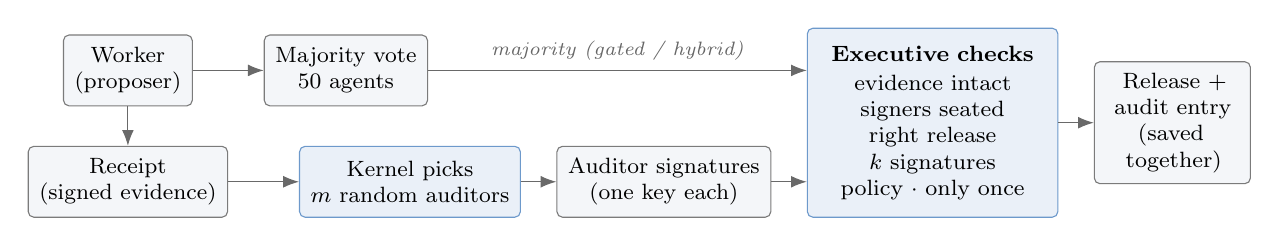
\begin{tikzpicture}[
      node distance=5mm and 4.5mm,
      box/.style={draw=headinggray!70, fill=panel, rounded corners=2pt, align=center,
                  font=\footnotesize, inner sep=4pt, minimum height=9mm},
      kern/.style={box, fill=dscolor!10, draw=dscolor!70},
      lab/.style={font=\scriptsize\itshape, text=subheadgray},
      arr/.style={-{Latex[length=2mm]}, draw=headinggray!80}]
    \node[box] (worker) {Worker\\(proposer)};
    \node[box, below=of worker] (evidence) {Receipt\\(signed evidence)};
    \node[box, right=9mm of worker] (swarm) {Majority vote\\50 agents};
    \node[kern, right=9mm of evidence] (seat) {Kernel picks\\$m$ random auditors};
    \node[box, right=of seat] (att) {Auditor signatures\\(one key each)};
    \node[kern, right=of att, yshift=7.5mm, minimum height=24mm, text width=29mm] (exec)
      {\textbf{Executive checks}\\[1pt] evidence intact\\ signers seated\\ right release\\ $k$ signatures\\ policy $\cdot$ only once};
    \node[box, right=of exec, text width=17mm] (db) {Release +\\audit entry\\(saved\\together)};
    \draw[arr] (worker) -- (swarm);
    \draw[arr] (worker) -- (evidence);
    \draw[arr] (evidence) -- (seat);
    \draw[arr] (seat) -- (att);
    \draw[arr] (att) -- (att -| exec.west);
    \draw[arr] (swarm) -- node[lab, above] {majority (gated / hybrid)} (swarm -| exec.west);
    \draw[arr] (exec) -- (db);
  \end{tikzpicture}
  \caption{The kernel. A \emph{release} is a record in the database; a \emph{receipt} is signed evidence about a build or run; an auditor approves by \emph{signing} one exact release with its own key (an HMAC). The kernel checks only these mechanics; whether a release is actually safe is decided by the auditors (and, in some rules, by the majority vote).}
  \label{fig:kernel}
\end{figure}

The kernel ({\small\nolinkurl{fleet_witness/institution.py}}; Figure~\ref{fig:kernel}) has
four parts. The \textbf{legislature} sets the policy. A \textbf{proposer} (a
worker agent, plus the majority vote in some rules) submits a release. The
kernel picks $m$ \textbf{auditors} at random, and each approves by
\emph{signing}: it attaches a code computed with its own secret key (an HMAC),
tied to that exact release. The \textbf{executive} records the release and an
audit entry together, in one database transaction \citep{sqlite}. It does so
only if a proposal exists, the policy allows it, the evidence has not been
tampered with, at least $k$ different seated auditors signed this exact
release, and nothing was released for this case before. We write this rule as
\emph{$k$-of-$m$}. The kernel never decides whether evidence actually makes a
release safe. In our task, a build receipt can be genuine and still not show
that the release is safe. That judgement belongs to the auditors, and it is
where colluders attack.

\subsection{Testing the kernel exhaustively}\label{sec:verification}

We let a program try every possible sequence of up to six actions on the real
kernel ({\small\nolinkurl{fleet_witness/verify_institution.py}}), in a small world: one
case, three seated auditors (two signatures needed), one outsider, and 12
possible actions, including forged, outsider, mismatched and duplicate
signatures and repeated release attempts. After every step, the kernel's state
is compared with a separately written description of correct behaviour:
\textbf{S1} no release unless every condition holds; \textbf{S2} a release
attempt succeeds whenever every condition holds; \textbf{S3} at most one release
per case; \textbf{S4} every release has its audit entry. To check that this test
can fail, we also run it on seven broken kernels, each missing one check. This
is bounded testing, not a proof. The test world is smaller than the live
experiments, and the same team wrote the kernel and its description, so a
mistake shared by both could go unnoticed (Appendix~\ref{app:verification}).

\subsection{What the kernel guarantees}\label{sec:guarantees}

\begin{itemize}[tight]
  \item \textbf{G1 (the checks; tested within the bound).} Nothing is released
        unless a proposal exists, the policy allows it, the evidence is intact
        and at least $k$ different seated auditors signed that exact release. At
        most one release happens per case, and each one is logged. This covers
        the database only, not external systems or many cases running at once.
  \item \textbf{G2 (seat bound).} If honest auditors never approve a bad release,
        then a bad release needs at least $k$ colluders on its committee. So
        colluders can win at most as often as $k$ or more of them happen to be
        seated.
  \item \textbf{G3 (probability).} If $m$ seats are drawn at random from $N$
        agents, $C$ of whom are colluders, if honest auditors make independent
        mistakes at rate $\varepsilon$, and if colluders always follow their
        plan, then the chance that a committee is captured is
\end{itemize}
\begin{equation}
  P(\text{capture}) \;=\; \sum_{j=0}^{m}
  \frac{\binom{C}{j}\binom{N-C}{m-j}}{\binom{N}{m}}\;
  \Pr\!\left[\operatorname{Bin}(m-j,\,\varepsilon) \ge k-j\right].
  \label{eq:g3}
\end{equation}
Colluders who sometimes disobey make capture less likely; honest auditors who
make the \emph{same} mistakes make it more likely than G3 says. Experiment~1
tests G1 and G2. Honest auditors almost never erred there, so G3's
independence assumption is tested in Experiment~2.

\subsection{Experiment 1: a checklist task}\label{sec:exp1}

Each run has 24 release requests. Eight are valid. Twelve are \textbf{targets}:
their receipts are genuine but prove the wrong thing (a build instead of a
safety review, or a different artifact or run), which honest agents can spot by
comparing fields. Four have forged receipts, which only the kernel can detect.
Fifty reviewers vote in five waves. In the \emph{visible} condition, later
waves see the running tally and recent comments; in the \emph{hidden}
condition, they do not. A hidden group of 0--50\% of the agents pushes the
targets using a shared talking point. For every case, the kernel draws seven
random seats, and an $m$-seat committee uses the first $m$. The same votes and
signatures are then judged under eight decision rules: direct majority; gated
majority (majority plus the kernel's checks); committees of 1-of-1, 2-of-3,
3-of-5, 4-of-7 and 7-of-7; and a hybrid (majority and 4-of-7). We ran DeepSeek
v4 Flash and gpt-oss-20b with the same random seeds, for 32,830 responses in
total (Appendix~\ref{app:supplementary} has the full setup and extra checks).

\subsection{Experiment 2: a judgement task}\label{sec:exp2}

In Experiment~1, agents only had to compare fields, which a program could do,
and honest agents almost never made mistakes. Experiment~2 uses a task that
needs judgement: \textbf{reviewing pull requests for hidden harmful code}, a job
AI agents already do for each other.

\head{Cases.}We wrote 48 pull requests to a small payments service. Each has a
title, the author's description, the code changes and a signed CI receipt.
Sixteen are safe; six of these look risky, such as a \code{subprocess} call with
fixed arguments. Twenty-four are harmful, at three difficulty levels: easy (a
hard-coded secret key), medium (a redirect to any address a user supplies) and
hard (a ``cleanup'' that makes signature checks vulnerable to timing attacks).
Eight are safe code with a forged CI receipt, which only the kernel can catch.
Each label rests on one specific behaviour, written down in advance. A model
that neither wrote the cases nor served as an agent (Meta Muse Wonder) labelled
every case without seeing our labels and agreed on 47 of 48. Like real pull
requests, each case bundles its change with two routine, safe edits. A small
pilot showed that single changes were too easy, and our plan allowed this one
difficulty adjustment.

\head{Reviewers and policy.}All reviewers and auditors get one policy: approve
only if the change does what its description says and adds no security,
data-exposure, safety-check or test-integrity risk. We ran two parts.
(i)~\emph{Honest judgement}: 12 reviewers and a 7-seat committee per case, no
colluders and a hidden board, with two frontier models (GPT-6.1 Sol and Gemini 4
Argon) and the two Experiment~1 models. (ii)~\emph{Colluder attack}: the full
50-agent setup of Experiment~1 with the two low-cost models, 0, 20 or 40\%
colluders pushing the 24 harmful changes with a code-review talking point,
visible and hidden boards, and all eight decision rules run through the kernel.
We did not use Claude models as agents, because Claude wrote the cases.

\head{Shared blind spots.}A random committee is safe only if honest reviewers
make independent mistakes, so that several of them rarely get the same case
wrong. For each case, we compute exactly how likely a $k$-of-$m$ committee drawn
from that case's honest reviews is to approve a harmful change (or block a safe
one). We compare the average with what independent mistakes at the same overall
rate would predict. A gap means mistakes cluster on the same changes: a shared
blind spot. We also compare which cases each model gets wrong, and test mixed
committees. Uncertainty comes from resampling the cases.

% =====================================================================
\section{Results}
% =====================================================================

\subsection{Testing the kernel}

The test explored 23,376 distinct states and 105,708 steps, and S1--S4 held
throughout. It caught all seven broken kernels, each within four to six actions
(Table~\ref{tab:verification}). One broken kernel, which allowed two releases
per case, was caught only at six actions and missed at five, which shows why
the test depth matters.

\subsection{Experiment 1: automatic checks and the seat bound}

\head{Automatic checks, not voting, stopped forgeries.}The direct majority
approved every forged release (48 of 48 per model), while every rule that used
the kernel blocked them all (Table~\ref{tab:main}). Agents cannot check a
signature, so the fair comparison is the \emph{gated majority}: the same votes
plus the kernel's checks. It released none of the 120 targets and none of the 48
forgeries, and all 96 valid releases, in each model. On this task, committees
added no safety over a gated majority.

\head{Committees failed only where seating allowed.}Honest auditors never
approved a target (0 of 746 per model), so every success for the colluders
came from colluders who happened to be seated. Captures never exceeded the seat
bound (G2) in any condition (Figure~\ref{fig:capture},
Appendix~\ref{app:supplementary}). A 4-of-7 committee was captured on 16 and 17
of 120 targets (95\% intervals 9--24 and 10--25), including when it never saw the
vote. Unanimity was never captured but blocked 9 of 96 valid gpt-oss releases.

\subsection{Experiment 2: judgement and shared blind spots}

\begin{table}[t]
  \centering\small
  \setlength{\tabcolsep}{4pt}
  \renewcommand{\arraystretch}{1.12}
  \caption{Honest reviewers on the 48 pull requests (no colluders, hidden board). Harmful approved: share of votes approving one of the 24 harmful changes. Safe blocked: share rejecting one of the 15 uncontested safe changes. Last two columns: chance that a random 4-of-7 committee of that model approves a harmful change, as observed (with 95\% interval) and as predicted if mistakes were independent.}
  \label{tab:honest}
  \begin{tabular}{@{}lrrcrr@{}}
    \toprule
    & \textbf{Harmful} & \textbf{Safe} & \textbf{Harmful cases}
    & \multicolumn{2}{c}{\textbf{4-of-7 committee approves harmful}} \\
    \cmidrule(l){5-6}
    \textbf{Model (votes per case)} & \textbf{approved} & \textbf{blocked} & \textbf{with any error}
    & \textbf{Observed} & \textbf{If independent} \\
    \midrule
    GPT-6.1 Sol (12)        & 0.0\%  & 0.0\%  & 0/24 & 0.0\% & 0.0\% \\
    Gemini 4 Argon (12)     & 0.0\%  & 0.6\%  & 0/24 & 0.0\% & 0.0\% \\
    DeepSeek v4 Flash (50)  & 0.1\%  & 0.4\%  & 1/24 & 0.0\% & 0.0\% \\
    gpt-oss-20b (50)        & \bad{12.0\%} & 6.4\% & 7/24 & \bad{12.0\%} {\footnotesize [0.4, 26.1]} & 0.5\% \\
    \addlinespace[2pt]
    Mixed DeepSeek + gpt-oss & -- & -- & -- & 0.1\% & -- \\
    \bottomrule
  \end{tabular}
\end{table}

\head{The task needs judgement.}A standard code-security scanner (Bandit)
flagged 5 of the 8 easy harmful changes and none of the 16 medium or hard ones,
with no false alarms (Appendix~\ref{app:exp2}).

\head{Frontier reviewers made no mistakes on harmful changes.}GPT-6.1 Sol and
Gemini 4 Argon rejected all 24 harmful changes in every review, and DeepSeek
erred once in 1,200 (Table~\ref{tab:honest}).

\head{A small model's mistakes landed on the same changes.}gpt-oss-20b approved
12\% of harmful changes, but not at random. All its mistakes fell on 7 of the 24,
and on three of them most of its reviewers approved: a rate limit that clients
can bypass by faking a header, an error handler that marks failed payments as
paid, and a test rewritten to accept a bug. So bigger committees did not help:
2-of-3, 3-of-5 and 4-of-7 committees all approved about 12\% of harmful changes,
the same as one reviewer. Independent mistakes would predict 4.0\%, 1.4\% and
0.5\%, although with only 7 error-prone cases the 95\% interval for 4-of-7 is
wide (0.4--26\%). This is the shared-blind-spot effect described by \citet{eckhardt1985}
and \citet{kim2025}.

\head{A stronger second model removes the blind spot.}Committees that mix
gpt-oss with DeepSeek (at least half the seats DeepSeek) approved harmful
changes 0.1\% of the time. DeepSeek alone was already near zero, so this shows
the value of seats held by a model without the same blind spots, not of
diversity as such. The cases each model got wrong correlated at 0.42 between
DeepSeek and gpt-oss, and hardly at all for Gemini.

\head{A contested case.}One safe change runs \code{git} when the program starts,
to report which version is deployed. DeepSeek, GPT-6.1 Sol and gpt-oss
reviewers rejected it (``startup fails if git is missing''), while Gemini
approved it unanimously. Both views are reasonable, so we report it as
contested rather than as a mistake and leave it out of the safe-change rates.

\head{The colluder attack.}Table~\ref{tab:exp2swarm} repeats the eight decision
rules on the judgement task with 20\% and 40\% colluders. For DeepSeek, the
pattern matches Experiment~1. Honest reviewers rejected every harmful change, so
every unsafe release came from seated colluders: 21 of 96 for a single auditor,
5 for 4-of-7, and none for unanimity or the hybrid. For gpt-oss, the gated
majority released 10 of 96 harmful changes. But comparing each decision with
what the honest agents decided on their own (no answer key needed) shows that
colluders flipped only 3 of 98 honest rejections. The rest were the honest
agents' own shared mistakes. Unanimity cut gpt-oss's unsafe releases to 5 of 96
but blocked 46 of 64 valid changes. Seeing the board \emph{lowered} honest gpt-oss approvals of
harmful changes, from 12.0\% to 6.3\% without colluders, and the colluders'
comments added back only about one percentage point.

\begin{table}[t]
  \centering\small
  \setlength{\tabcolsep}{4pt}
  \renewcommand{\arraystretch}{1.1}
  \caption{Experiment 2 colluder attack (20\% and 40\% colluders, both boards). Unsafe: harmful changes released (of 96). Flipped: releases of changes most honest agents rejected in the matching run without colluders (of 100 and 98; no answer key needed). Valid: safe changes released (of 64). Kernel rules released 0 of 32 forgeries; the direct majority 31 and 29.}
  \label{tab:exp2swarm}
  \begin{tabular}{@{}l rr rr rr@{}}
    \toprule
    & \multicolumn{2}{c}{\textbf{Unsafe}} & \multicolumn{2}{c}{\textbf{Flipped}}
    & \multicolumn{2}{c}{\textbf{Valid}} \\
    \cmidrule(lr){2-3}\cmidrule(lr){4-5}\cmidrule(lr){6-7}
    \textbf{Decision rule} & DS & GPT & DS & GPT & DS & GPT \\
    \midrule
    Direct / gated majority   & 0 & 10 & 0 & 3 & 59 & 54 \\
    Auditor 1-of-1            & 21 & 24 & 21 & 19 & 57 & 43 \\
    Committee 2-of-3          & 8 & 12 & 8 & 8 & 59 & 50 \\
    Committee 3-of-5          & 7 & 8 & 7 & 3 & 58 & 51 \\
    Committee 4-of-7          & 5 & 9 & 5 & 4 & 58 & 52 \\
    Unanimous 7-of-7          & \good{0} & 5 & 0 & 0 & 51 & \bad{18} \\
    Hybrid (majority \& 4-of-7) & \good{0} & 7 & 0 & 2 & 58 & 52 \\
    \bottomrule
  \end{tabular}
\end{table}

% =====================================================================
\section{Discussion and Limitations}
% =====================================================================

\head{Verify the institution, not the agents.}We never verified a single agent.
Still, no forgery got through, and colluders won only as often as seating
allowed, as long as honest reviewers were reliable. When reviewers share blind
spots, adding more copies of the same model adds nothing, and the idea that more
judges are safer breaks down \citep{ladha1992}. The practical rules are: put
everything a program can check into the kernel; for each task, measure how often
honest reviewers make mistakes and whether they make the same ones; and where
they do, seat reviewers that do not share those blind spots. A companion pilot
agrees (Appendix~\ref{app:pilot}): a live supervisor swung from unsafe approvals
to refusing everything, while the controller blocked every invalid action.

\head{Limitations.}G2 and G3 assume reliable, independent honest reviewers,
which the small model was not. Our colluders did not attack the seating, the
keys or the kernel itself. The kernel test is bounded, not a proof. Both tasks
are synthetic and written by us; one independent model checked our labels (47
of 48 agreed). Colluders coordinated only through a shared
plan and the public board, with no private channel, no division of tasks and no
change of plan. The colluder attack used two low-cost models; frontier models
were tested only as honest reviewers. We changed one prompt after stopping a
first run (Appendices~\ref{app:limitations}, \ref{app:provenance}, \ref{app:exp2}).

\head{Future work: contested questions.}Where there is no single right answer,
as in our contested case, an institution must be judged by whether it matches
its honest members and resists takeover. Next: contested cases targeted by colluders, swarms that talk
privately or adapt to who is seated, and a kernel at a real MCP or A2A gateway.

% =====================================================================
\section{Conclusion}
% =====================================================================

A small, verifiable institution stopped every forged release, and its committees
failed only as often as seating allowed while honest reviewers were reliable.
When they were not, seven copies of one model were no safer than one. AI
institutions can be built and tested today; their committees are only as safe as
their reviewers' blind spots are different.

% =====================================================================
%  References
% =====================================================================
\begingroup
\setlength{\parskip}{0pt}
\renewcommand{\bibsection}{\section*{References}}
\setlength{\bibsep}{3pt}
\small
\begin{thebibliography}{99}

\bibitem[Apart Research(2026)]{apart2026}
Apart Research (2026). \emph{Swarm Alignment Hackathon}: brief and resources.
\url{https://apartresearch.com/sprints/swarm-alignment-2026}

\bibitem[Deochake(2026)]{deochake2026}
Deochake, S. (2026). Heartbeat-bound hierarchical credentials: Cryptographic
revocation for AI agent swarms. \arxiv{2605.20704}.

\bibitem[Desmedt and Frankel(1989)]{desmedt1989}
Desmedt, Y.\ and Frankel, Y. (1989). Threshold cryptosystems. In
\emph{Advances in Cryptology -- CRYPTO '89}.

\bibitem[Dolan-Gavitt et~al.(2016)]{dolangavitt2016}
Dolan-Gavitt, B., et al. (2016). LAVA: Large-scale automated vulnerability
addition. In \emph{IEEE Symposium on Security and Privacy}.

\bibitem[Eckhardt and Lee(1985)]{eckhardt1985}
Eckhardt, D.\,E.\ and Lee, L.\,D. (1985). A theoretical basis for the analysis of
multiversion software subject to coincident errors. \emph{IEEE Transactions on
Software Engineering}, SE-11(12).

\bibitem[Gilad et~al.(2017)]{gilad2017}
Gilad, Y., et al. (2017). Algorand: Scaling Byzantine agreements for
cryptocurrencies. In \emph{Proceedings of the 26th ACM Symposium on Operating
Systems Principles (SOSP)}.

\bibitem[Greenblatt et~al.(2024)]{greenblatt2024}
Greenblatt, R., et al. (2024). AI control: Improving safety despite intentional
subversion. \arxiv{2312.06942}.

\bibitem[Hammond et~al.(2025)]{hammond2025}
Hammond, L., et al. (2025). Multi-agent risks from advanced AI.
\arxiv{2502.14143}.

\bibitem[Kekatos et~al.(2026)]{kekatos2026}
Kekatos, N., et al. (2026). Mission-level runtime assurance for LLM-assisted ISR
swarms over a verification-aware fabric. \arxiv{2607.23532}.

\bibitem[Kim et~al.(2025)]{kim2025}
Kim, E., et al. (2025). Correlated errors in large language models.
\arxiv{2506.07962}.

\bibitem[Knight and Leveson(1986)]{knight1986}
Knight, J.\,C.\ and Leveson, N.\,G. (1986). An experimental evaluation of the
assumption of independence in multiversion programming. \emph{IEEE Transactions
on Software Engineering}, SE-12(1).

\bibitem[Ladha(1992)]{ladha1992}
Ladha, K.\,K. (1992). The Condorcet jury theorem, free speech, and correlated
votes. \emph{American Journal of Political Science}, 36(3).

\bibitem[Lamport et~al.(1982)]{lamport1982}
Lamport, L., Shostak, R.\ and Pease, M. (1982). The Byzantine generals problem.
\emph{ACM Transactions on Programming Languages and Systems}, 4(3).

\bibitem[Motwani et~al.(2024)]{motwani2024}
Motwani, S., et al. (2024). Secret collusion among AI agents: Multi-agent
deception via steganography. In \emph{Advances in Neural Information Processing
Systems (NeurIPS)}.

\bibitem[Muruaga(2026)]{muruaga2026}
Muruaga, X. (2026). Bounded Agents: Delegation security for multi-agent AI
systems. \arxiv{2608.15888}.

\bibitem[Nguyen and Tran(2026)]{nguyen2026}
Nguyen, H.-D.\ and Tran, X.-T. (2026). Verify-gated completion as admission
control in a governed multi-agent runtime: A bounded architecture case study.
\arxiv{2605.17998}.

\bibitem[Paglieri et~al.(2026)]{paglieri2026}
Paglieri, D., et al. (2026). A case study on emergent cheating and
whistleblowing in autonomous research swarms. \arxiv{2609.04170}.

\bibitem[Ruan(2026)]{ruan2026}
Ruan, A. (2026). From logic monopoly to social contract: Separation of power and
the institutional foundations for autonomous agent economies.
\arxiv{2603.25100}.

\bibitem[SQLite(n.d.)]{sqlite}
SQLite (n.d.). Atomic commit in SQLite. \url{https://sqlite.org/atomiccommit.html}

\bibitem[Wang(2026)]{wang2026}
Wang, Z. (2026). Proof-carrying agent actions: Model-agnostic runtime governance
for heterogeneous agent systems. \arxiv{2606.04104}.

\bibitem[Zheng and Zhang(2026)]{zheng2026}
Zheng, S.\ and Zhang, Q. (2026). AgentRFC: Security design principles and
conformance testing for agent protocols. \arxiv{2603.23801}.

\end{thebibliography}
\endgroup

% =====================================================================
%  Back matter and appendices
% =====================================================================
\setcounter{section}{0}
\renewcommand{\thesection}{\Alph{section}}
\renewcommand{\theHsection}{appendix.\Alph{section}}

\section*{Code and Data}

\begin{itemize}[tight]
  \item \textbf{Code repository:} \url{https://github.com/k2jac9/fleet-witness},
        containing the kernel, bounded checker, swarm harness, analysis and
        figure scripts, and tests.
  \item \textbf{Data:} every reported run, including the superseded truncated
        run and the 600-token pilot, is published as
        \code{data/fleet-witness-runs-2026-11-08.zip}: public event logs, sealed
        ground truth, per-regime decisions and run manifests (see
        \code{data/README.md}).
  \item \textbf{Reproduction:} \code{scripts/reproduce\_tables.py} recomputes
        every table offline from the archive, and \code{scripts/rigor\_stats.py}
        computes the board splits, draw-level intervals, seat-bound
        opportunities, detector counts and truncation comparison; neither makes
        model calls.
  \item \textbf{Experiment 2:} plan and plan review in
        {\small\nolinkurl{docs/report/JUDGEMENT_PLAN.md}}; cases in
        {\small\nolinkurl{fleet_witness/swarm/judgement_cases.py}}; runs via
        {\small\nolinkurl{scripts/judgement_experiment.py}}; analysis in
        {\small\nolinkurl{scripts/judgement_analysis.py}},
        {\small\nolinkurl{label_check.py}} and {\small\nolinkurl{bandit_baseline.py}}.
  \item \textbf{Companion pilot:} the live-supervisor pilot (Appendix~\ref{app:pilot})
        is reported in full in {\small\nolinkurl{docs/report/latest.md}}, with its
        evidence package in {\small\nolinkurl{docs/submission/latest/}}.
  \item \textbf{Timeline:} Experiment 1 runs finished on 2026-11-08 (latest
        manifest timestamp 2026-11-09 02:07 UTC). Experiment 2 ran on 2026-11-09
        between 08:30 and 09:10 UTC, i.e.\ 2026-11-08 AoE, before the 23:59 AoE
        deadline.
\end{itemize}

\section*{Author Contributions}

A.C.\ built the Fleet Witness baseline (trusted controller, scripted evaluation,
replay viewer and cloud deployment) that this work extends, and led the
statistical correction and provenance review, the controlled paid-run
infrastructure, and the live-supervisor pilot (Appendix~\ref{app:pilot}). I.P.B.\
proposed the institutional-verification research direction, and designed and ran
the institution kernel, bounded verification and both swarm experiments with AI
coding assistance. Both authors are responsible for the final manuscript.

% ---------------------------------------------------------------------
\appendixsection{Limitations and Dual-Use / Ethical Considerations}\label{app:limitations}

\subsection*{A.1 Limitations}

\begin{itemize}[tight]
  \item \textbf{Bounded, not complete.} The kernel test covers one case, three
        seats and up to six actions. Larger worlds and many cases running at once
        are untested. The same team wrote the kernel and the description it is
        checked against, so a mistake shared by both would go unnoticed.
  \item \textbf{Synthetic tasks and planted colluders.} Both tasks were written by
        us. Colluders were told what to do; their coordination did not emerge on
        its own, and they had no private channel, no division of tasks and no
        way to change plan during a run.
  \item \textbf{Models.} The colluder attacks used two low-cost models (DeepSeek
        v4 Flash and gpt-oss-20b); GPT-6.1 Sol and Gemini 4 Argon were tested
        only as honest reviewers. Qwen 3.7 Flash was dropped after a pilot (logs
        not kept) in which it used its whole 600-token budget on hidden reasoning
        in about 39\% of responses; at 2,000 tokens it was too slow. A second
        provider (Adaption) was tried in a pilot but was too rate-limited.
  \item \textbf{Small samples.} Experiment~1 has 12 committee draws per colluder
        share, each used under both boards and both models; we report intervals
        at the level of draws and make no significance claims. Experiment~2 has 48
        pull requests, and its committee results rest on the 7 harmful changes
        that gpt-oss got wrong.
  \item \textbf{Honest mistakes.} In Experiment~1, honest auditors never approved a
        target (0 of 746 per model), and near-miss receipts produced almost no
        mistakes either (Table~\ref{tab:nearmiss}), so independence could only be
        tested in Experiment~2. There, mistakes clustered strongly for gpt-oss;
        the frontier models made too few mistakes on harmful changes to test it.
  \item \textbf{Labels.} One independent model checked our 48 labels (47 agreed).
        One case was contested between models and is reported separately. Other
        labels could still be wrong.
  \item \textbf{Seating.} Committees were drawn by a seeded random generator that
        colluders could not see. Colluders who can predict or influence seating
        would break the seat bound.
  \item \textbf{Keys and trust.} The kernel's keys and database are trusted.
        Signatures use shared-secret codes (HMAC) checked only by the kernel, so
        outsiders cannot verify them and a compromised host is not covered. Keys
        are created fresh for each run; rotating, revoking and recovering keys are
        not implemented. Public-key signatures (e.g.\ Ed25519), credential
        revocation \citep{deochake2026} and tamper-evident logs would keep the same
        rules while allowing outside audits. Containers and operating-system
        isolation are out of scope.
  \item \textbf{Records.} Experiment~1's run records lack the exact code version,
        temperature and provider request IDs, and most lack retry information
        (Appendix~\ref{app:provenance}). Experiment~2 ran outside the
        repository's gated paid workflow (Appendix~\ref{app:exp2}).
\end{itemize}

\subsection*{A.2 Dual-use}

\textit{Could this make multi-agent operations easier, or harder to detect?}
\begin{itemize}[tight]
  \item \textbf{Easier:} the harness creates instructed colluding agents and
        measures committee capture, so an attacker could use the capture curves
        to size a cell. The kernel's rules are public, so its blind spot is also
        known: it trusts auditors on semantic judgements.
  \item \textbf{Harder to detect:} a colluder who knew about the output-length
        association or the shared-minority detector could try to evade them.
  \item \textbf{Overall:} we judge that the work favours defenders. It shows that
        mechanical checks block forgery outright, that committee risk is
        predictable, and how to detect a planted cell.
\end{itemize}
Mitigations: the task is synthetic and nothing touches third-party systems;
there is no scanning, recruitment or contact with real agents; the talking points
are generic; and the detector and the output-length association are published
alongside, favouring defenders.

\subsection*{A.3 Ethics and provenance of work}

There are no human subjects and no personal data. The repository was created
during the sprint (2026-11-08); earlier conceptual research informed the design,
but no pre-sprint code is used (\code{docs/AI\_ASSISTANCE.md}). The scripted
Fleet Witness controller was built earlier in the same sprint; the institution
kernel, checker and swarm harness were built after it. AI assistance is
described in the LLM Usage Statement.

% ---------------------------------------------------------------------
\appendixsection{Verification and Audit Details}\label{app:verification}

\subsection*{B.1 The test world}

One case, three seated auditors (two signatures needed) and one registered but
unseated agent; the evidence is either intact or tampered with. The 12 actions
are: a proposal with or without majority support; policy on or off; a valid
signature from each seat and from the outsider; a forged signature; a signature
for the wrong artifact; and two separate release attempts. Repeating an action
models duplicates and replays. The test explores states in order of depth,
saving and copying the database at each step and skipping states it has already
seen. Both kernel modes (committee only, and committee plus majority) are
checked.

\subsection*{B.2 Verification results}

\begin{table}[H]
  \centering\small
  \renewcommand{\arraystretch}{1.1}
  \caption{Kernel test results. For each broken kernel, the last column gives the
    shortest sequence of actions that exposed it, from the saved test output.}
  \label{tab:verification}
  \begin{tabular}{@{}llc@{}}
    \toprule
    \textbf{Check} & \textbf{Result} & \textbf{Counterexample} \\
    \midrule
    Kernel, depth 6               & 23,376 states, 105,708 transitions; S1--S4 hold & -- \\
    Committee-only mode, depth 4  & 3,188 states; all hold & -- \\
    Hybrid mode, depth 4          & 2,906 states; all hold & -- \\
    \midrule
    Broken: skip policy recheck   & Caught, S1 & 4 actions \\
    Broken: skip integrity        & Caught, S1 (tampered evidence) & 5 actions \\
    Broken: skip seat check       & Caught, S1 (outsider attests) & 5 actions \\
    Broken: skip binding          & Caught, S1 (wrong-artifact attestation) & 5 actions \\
    Broken: count duplicates      & Caught, S1 (same auditor twice) & 5 actions \\
    Broken: skip uniqueness       & Caught, S3 (two releases; missed at depth 5) & 6 actions \\
    Broken: skip audit            & Caught, S4 & 5 actions \\
    \bottomrule
  \end{tabular}
\end{table}

\subsection*{B.3 Cut-off responses in Experiment 1}

For gpt-oss, no saved response reached the 2,000-token limit (the longest was
1,536 tokens). For DeepSeek, one colluder response hit the limit in the 30\% run.
Under a rule we set before seeing results, we re-ran that whole run with retries
turned on; no retries were needed. Across all eight decision rules and both
boards, 15 of 16 results were identical; the only change was the 4-of-7 hidden-
board result (one capture became zero). Both runs are kept
(\code{runs/deepseek2k-f30-truncated}, \code{runs/sweep-deepseek2k/f30}), and
the main results use the re-run. The archive does not timestamp the rule, and
missing retry fields elsewhere mean we cannot rule out other cut-off attempts.

\subsection*{B.4 Colluder detector (Experiment 1)}\label{app:detector}

The detector reads only public votes and reasons. For each pair of agents it
measures how often both voted on the losing side, and how similar their written
reasons are (TF-IDF cosine similarity). Both measures are turned into robust
$z$-scores. A pair is linked if the average of the two scores is at least 2.0,
the losing-side score is at least 3.0, and they shared at least one losing vote.
Groups of three or more linked agents are flagged. The settings were tuned on
scripted runs before the live experiments (code:
\code{fleet\_witness/swarm/detect.py}). It found the planted group with no false
positives at any non-zero colluder share (Table~\ref{tab:detector}), but only
because the group shared a talking point and lost its votes.

\begin{table}[H]
  \centering\small
  \renewcommand{\arraystretch}{1.1}
  \caption{Detector confusion counts, summed over both board conditions; the unit
    is an agent in one run condition. At 0\% there are no colluders, so every
    flagged agent is a false positive.}
  \label{tab:detector}
  \begin{tabular}{@{}l ccc ccc@{}}
    \toprule
    & \multicolumn{3}{c}{\textbf{DeepSeek}} & \multicolumn{3}{c}{\textbf{gpt-oss}} \\
    \cmidrule(lr){2-4}\cmidrule(lr){5-7}
    \textbf{Colluder share} & TP & FP & FN & TP & FP & FN \\
    \midrule
    0\%  & -- & 0 & -- & -- & 3 & -- \\
    10\% & 10 & 0 & 0 & 10 & 0 & 0 \\
    20\% & 20 & 0 & 0 & 20 & 0 & 0 \\
    30\% & 30 & 0 & 0 & 30 & 0 & 0 \\
    40\% & 40 & 0 & 0 & 39 & 0 & 1 \\
    50\% & 49 & 0 & 1 & 48 & 0 & 2 \\
    \bottomrule
  \end{tabular}
\end{table}

% ---------------------------------------------------------------------
\appendixsection{Experiment 1: Supplementary Results}\label{app:supplementary}

\begin{figure}[H]
  \centering
  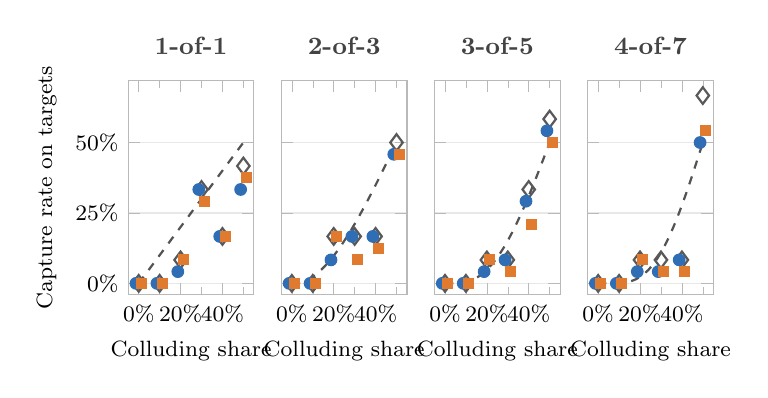
\begin{tikzpicture}
    \begin{groupplot}[fwplot,
        group style={group size=4 by 1, horizontal sep=0.35cm, y descriptions at=edge left},
        width=0.262\textwidth, height=4.3cm,
        xmin=-5, xmax=55, ymin=-4, ymax=72,
        xtick={0,20,40}, minor xtick={10,30,50}, ytick={0,25,50},
        xticklabel={\pgfmathprintnumber{\tick}\%}, yticklabel={\pgfmathprintnumber{\tick}\%},
        xlabel={Colluding share}]
      \nextgroupplot[title={1-of-1}, ylabel={Capture rate on targets}, legend to name=caplegend]
        \addplot[thick, dashed, gray!65!black] coordinates {(0,0) (2,2) (4,4) (6,6) (8,8) (10,10) (12,12) (14,14) (16,16) (18,18) (20,20) (22,22) (24,24) (26,26) (28,28) (30,30) (32,32) (34,34) (36,36) (38,38) (40,40) (42,42) (44,44) (46,46) (48,48) (50,50)};
        \addlegendentry{A-priori probability (G3)}
        \addplot[only marks, mark=diamond, mark size=3pt, thick, gray!70!black] coordinates {(0,0) (10,0) (20,8.33) (30,33.33) (40,16.67) (50,41.67)};
        \addlegendentry{Seat bound for the draws (G2)}
        \addplot[only marks, mark=*, mark size=2.1pt, dscolor] coordinates {(-1.3,0) (8.7,0) (18.7,4.17) (28.7,33.33) (38.7,16.67) (48.7,33.33)};
        \addlegendentry{Observed, DeepSeek}
        \addplot[only marks, mark=square*, mark size=1.8pt, gptcolor] coordinates {(1.3,0) (11.3,0) (21.3,8.33) (31.3,29.17) (41.3,16.67) (51.3,37.5)};
        \addlegendentry{Observed, gpt-oss}
      \nextgroupplot[title={2-of-3}]
        \addplot[thick, dashed, gray!65!black] coordinates {(0,0) (2,0) (4,0.24) (6,0.72) (8,1.43) (10,2.35) (12,3.47) (14,4.79) (16,6.29) (18,7.96) (20,9.80) (22,11.79) (24,13.92) (26,16.18) (28,18.57) (30,21.07) (32,23.67) (34,26.37) (36,29.14) (38,31.99) (40,34.90) (42,37.86) (44,40.86) (46,43.89) (48,46.94) (50,50)};
        \addplot[only marks, mark=diamond, mark size=3pt, thick, gray!70!black] coordinates {(0,0) (10,0) (20,16.67) (30,16.67) (40,16.67) (50,50)};
        \addplot[only marks, mark=*, mark size=2.1pt, dscolor] coordinates {(-1.3,0) (8.7,0) (18.7,8.33) (28.7,16.67) (38.7,16.67) (48.7,45.83)};
        \addplot[only marks, mark=square*, mark size=1.8pt, gptcolor] coordinates {(1.3,0) (11.3,0) (21.3,16.67) (31.3,8.33) (41.3,12.5) (51.3,45.83)};
      \nextgroupplot[title={3-of-5}]
        \addplot[thick, dashed, gray!65!black] coordinates {(0,0) (2,0) (4,0) (6,0.05) (8,0.20) (10,0.48) (12,0.92) (14,1.56) (16,2.42) (18,3.50) (20,4.83) (22,6.40) (24,8.22) (26,10.30) (28,12.62) (30,15.17) (32,17.95) (34,20.94) (36,24.13) (38,27.49) (40,31.00) (42,34.64) (44,38.38) (46,42.21) (48,46.09) (50,50)};
        \addplot[only marks, mark=diamond, mark size=3pt, thick, gray!70!black] coordinates {(0,0) (10,0) (20,8.33) (30,8.33) (40,33.33) (50,58.33)};
        \addplot[only marks, mark=*, mark size=2.1pt, dscolor] coordinates {(-1.3,0) (8.7,0) (18.7,4.17) (28.7,8.33) (38.7,29.17) (48.7,54.17)};
        \addplot[only marks, mark=square*, mark size=1.8pt, gptcolor] coordinates {(1.3,0) (11.3,0) (21.3,8.33) (31.3,4.17) (41.3,20.83) (51.3,50)};
      \nextgroupplot[title={4-of-7}]
        \addplot[thick, dashed, gray!65!black] coordinates {(0,0) (2,0) (4,0) (6,0) (8,0.02) (10,0.07) (12,0.20) (14,0.45) (16,0.85) (18,1.45) (20,2.28) (22,3.38) (24,4.77) (26,6.49) (28,8.53) (30,10.91) (32,13.64) (34,16.70) (36,20.08) (38,23.75) (40,27.69) (42,31.86) (44,36.22) (46,40.73) (48,45.34) (50,50)};
        \addplot[only marks, mark=diamond, mark size=3pt, thick, gray!70!black] coordinates {(0,0) (10,0) (20,8.33) (30,8.33) (40,8.33) (50,66.67)};
        \addplot[only marks, mark=*, mark size=2.1pt, dscolor] coordinates {(-1.3,0) (8.7,0) (18.7,4.17) (28.7,4.17) (38.7,8.33) (48.7,50)};
        \addplot[only marks, mark=square*, mark size=1.8pt, gptcolor] coordinates {(1.3,0) (11.3,0) (21.3,8.33) (31.3,4.17) (41.3,4.17) (51.3,54.17)};
    \end{groupplot}
  \end{tikzpicture}

  \vspace{2pt}
  \ref*{caplegend}
  \caption{Capture rate on target releases by colluding share for the four
    capturable committee regimes. Each observed point is 24 paired outcomes from
    12 committee draws. Diamonds show the seat bound realized by those draws
    (G2); dashed lines show the a-priori probability (Eq.~\ref{eq:g3},
    $N = 50$, $\varepsilon = 0$). No observed point exceeds its diamond. The
    direct majority, gated majority, 7-of-7 and hybrid were never captured.}
  \label{fig:capture}
\end{figure}

\begin{table}[H]
  \centering\small
  \setlength{\tabcolsep}{3.2pt}
  \renewcommand{\arraystretch}{1.12}
  \caption{Outcomes by regime. \emph{Unsafe released} pools colluder shares
    10--50\% and both boards (120 paired target outcomes from 60 committee
    draws); \emph{valid} and \emph{forged released} pool all six shares
    including 0\% (6 shares $\times$ 2 boards $\times$ 8 or 4 cases).
    DS = DeepSeek v4 Flash, GPT = gpt-oss-20b. Seat bound and expectation are
    shared by both models (same seeds and committees); the expectation assumes
    $\varepsilon = 0$ and full colluder compliance. Requests per decision are
    nominal standalone requests, not measured costs.}
  \label{tab:main}
  \begin{tabular}{@{}l rr rr rr rrr@{}}
    \toprule
    & \multicolumn{2}{c}{\textbf{Unsafe released}}
    & \multicolumn{2}{c}{\textbf{Valid released}}
    & \multicolumn{2}{c}{\textbf{Forged released}}
    & \textbf{Seat} & \textbf{Expected} & \textbf{Requests} \\
    & \multicolumn{2}{c}{(of 120 targets)} & \multicolumn{2}{c}{(of 96)}
    & \multicolumn{2}{c}{(of 48)} & \textbf{bound} & \textbf{(G3)} & \textbf{/ decision}\\
    \cmidrule(lr){2-3}\cmidrule(lr){4-5}\cmidrule(lr){6-7}
    \textbf{Decision rule} & DS & GPT & DS & GPT & DS & GPT & \textbf{(G2)} & & \\
    \midrule
    Direct majority                & \good{0} & \good{0} & 96 & 96 & \bad{48} & \bad{48} & -- & -- & 50 \\
    Gated majority                 & \good{0} & \good{0} & 96 & 96 & \good{0} & \good{0} & -- & -- & 50 \\
    \addlinespace[2pt]
    Auditor 1-of-1                 & 21 & 22 & 96 & 95 & 0 & 0 & 24 & 36.0 & 1 \\
    Committee 2-of-3               & 21 & 20 & 96 & 96 & 0 & 0 & 24 & 28.3 & 3 \\
    Committee 3-of-5               & 23 & 20 & 96 & 96 & 0 & 0 & 26 & 24.4 & 5 \\
    Committee 4-of-7               & 16 & 17 & 96 & 96 & 0 & 0 & 22 & 21.8 & 7 \\
    Unanimous 7-of-7               & \good{0} & \good{0} & 96 & \bad{87} & 0 & 0 & 0 & 0.1 & 7 \\
    \addlinespace[2pt]
    Hybrid (majority \& 4-of-7)    & \good{0} & \good{0} & 96 & 96 & 0 & 0 & 22$^\dagger$ & 21.8$^\dagger$ & 57 \\
    \bottomrule
  \end{tabular}

  \vspace{4pt}
  \begin{minipage}{\textwidth}\footnotesize\setstretch{1}
    $^\dagger$\,Committee-only opportunity, not a hybrid prediction: the hybrid
    also needs a strict majority (approvals $>$ denials), which honest
    voters never gave a target. Draw-level intervals and splits: Appendix~\ref{app:supplementary}.
  \end{minipage}
\end{table}

\subsection*{C.1 Robustness of the committee results}

\begin{table}[H]
  \centering\small
  \renewcommand{\arraystretch}{1.1}
  \caption{Unsafe releases on targets by board condition (of 60 each), and 95\%
    intervals for the pooled count (of 120) from a stratified cluster bootstrap
    over committee draws (20,000 replicates; each draw keeps both board outcomes;
    resampling within colluder share). Regimes never captured are omitted.}
  \label{tab:robust}
  \begin{tabular}{@{}l ccc ccc@{}}
    \toprule
    & \multicolumn{3}{c}{\textbf{DeepSeek}} & \multicolumn{3}{c}{\textbf{gpt-oss}} \\
    \cmidrule(lr){2-4}\cmidrule(lr){5-7}
    \textbf{Regime} & Hidden & Visible & Total [95\% CI] & Hidden & Visible & Total [95\% CI] \\
    \midrule
    Auditor 1-of-1   & 10 & 11 & 21 [11, 32] & 10 & 12 & 22 [12, 33] \\
    Committee 2-of-3 & 10 & 11 & 21 [11, 31] &  9 & 11 & 20 [11, 30] \\
    Committee 3-of-5 & 10 & 13 & 23 [13, 33] & 10 & 10 & 20 [12, 29] \\
    Committee 4-of-7 &  7 &  9 & 16 [9, 24]  &  8 &  9 & 17 [10, 25] \\
    \bottomrule
  \end{tabular}
\end{table}

\begin{table}[H]
  \centering\small
  \renewcommand{\arraystretch}{1.1}
  \caption{Unsafe releases on targets by colluder share (of 24 per share and
    model: DeepSeek / gpt-oss), with the seat bound realized by the draws in
    parentheses. The gated majority, 7-of-7 and hybrid were never captured.}
  \label{tab:byshare}
  \begin{tabular}{@{}lcccc@{}}
    \toprule
    \textbf{Colluder share} & \textbf{1-of-1} & \textbf{2-of-3} & \textbf{3-of-5} & \textbf{4-of-7} \\
    \midrule
    10\% & 0 / 0 \ (0)  & 0 / 0 \ (0)    & 0 / 0 \ (0)    & 0 / 0 \ (0) \\
    20\% & 1 / 2 \ (2)  & 2 / 4 \ (4)    & 1 / 2 \ (2)    & 1 / 2 \ (2) \\
    30\% & 8 / 7 \ (8)  & 4 / 2 \ (4)    & 2 / 1 \ (2)    & 1 / 1 \ (2) \\
    40\% & 4 / 4 \ (4)  & 4 / 3 \ (4)    & 7 / 5 \ (8)    & 2 / 1 \ (2) \\
    50\% & 8 / 9 \ (10) & 11 / 11 \ (12) & 13 / 12 \ (14) & 12 / 13 \ (16) \\
    \midrule
    Total (of 120) & 21 / 22 \ (24) & 21 / 20 \ (24) & 23 / 20 \ (26) & 16 / 17 \ (22) \\
    \bottomrule
  \end{tabular}
\end{table}

\subsection*{C.2 Colluders wrote longer responses}

On target cases, colluders' responses were 1.9--2.8 times longer than honest
agents' (median output tokens, including hidden reasoning; Figure~\ref{fig:tokens}).
For DeepSeek: 106 vs 294 for votes and 110.5 vs 240.5 for audits; for gpt-oss: 158
vs 369 and 174 vs 327.5. Colluders also received a longer prompt with a
conflicting instruction, so this is a correlation, not a measured cost of lying,
and it may not hold for colluders who adapt.

\begin{figure}[H]
  \centering
  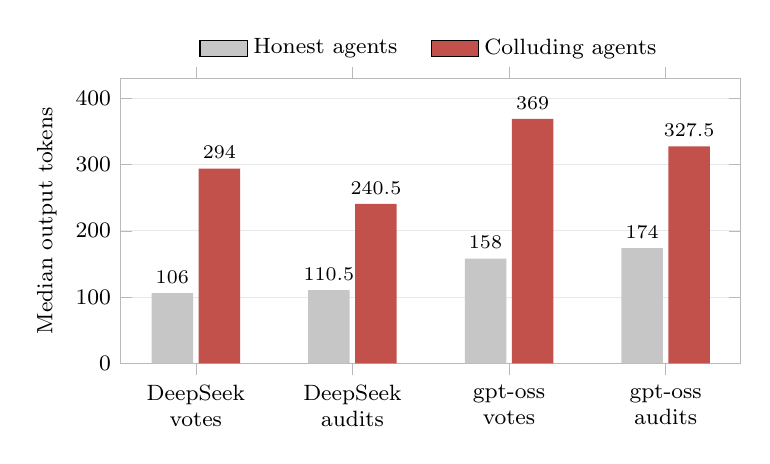
\begin{tikzpicture}
    \begin{axis}[fwplot,
        ybar, area legend, bar width=15pt, width=0.78\textwidth, height=5.2cm,
        enlarge x limits=0.16, ymin=0, ymax=430,
        symbolic x coords={dsv, dsa, gv, ga},
        xtick=data, xticklabels={{DeepSeek\\votes}, {DeepSeek\\audits}, {gpt-oss\\votes}, {gpt-oss\\audits}},
        xticklabel style={align=center},
        ylabel={Median output tokens},
        nodes near coords, every node near coord/.append style={font=\scriptsize},
        legend style={at={(0.5,1.03)}, anchor=south}]
      \addplot[fill=gray!45, draw=none] coordinates {(dsv,106) (dsa,110.5) (gv,158) (ga,174)};
      \addlegendentry{Honest agents}
      \addplot[fill=alertred!80, draw=none] coordinates {(dsv,294) (dsa,240.5) (gv,369) (ga,327.5)};
      \addlegendentry{Colluding agents}
    \end{axis}
  \end{tikzpicture}
  \caption{Colluding agents produced longer outputs. Median output tokens,
    including hidden reasoning, on target cases, by role and model (ratios
    1.9--2.8$\times$). Colluders also received a longer, conflicting prompt, so
    this is an association, not a measured cost of deception.}
  \label{fig:tokens}
\end{figure}

\subsection*{C.3 Honest error on near-miss releases}

\begin{table}[H]
  \centering\small
  \renewcommand{\arraystretch}{1.1}
  \caption{Honest error on near-miss releases in the zero-collusion cell: 108
    case-conditions per model, i.e.\ 756 auditor seats ($108 \times 7$). These
    are distinct from the 746 honest target seats of the main experiment.}
  \label{tab:nearmiss}
  \begin{tabular}{@{}lll@{}}
    \toprule
    & \textbf{DeepSeek} & \textbf{gpt-oss} \\
    \midrule
    Committee auditors (756 seats)              & 0.3\% (issuer capitalization only) & 0\% \\
    Reviewer votes                              & 1.0\%                              & 0\% \\
    Committees captured by honest error alone   & 1-of-1: 2/108; larger: 0           & 0 \\
    \bottomrule
  \end{tabular}
\end{table}

% ---------------------------------------------------------------------
\appendixsection{Retained Accounting and Provenance}\label{app:provenance}

\subsection*{D.1 Reproducibility statement}

\begin{table}[H]
  \centering\small
  \renewcommand{\arraystretch}{1.15}
  \caption{What can and cannot be reproduced from the published archive.}
  \label{tab:repro}
  \begin{tabularx}{\textwidth}{@{}>{\raggedright\arraybackslash}p{0.2\textwidth}X@{}}
    \toprule
    \textbf{Status} & \textbf{Items} \\
    \midrule
    Retained          & Per-agent votes, attestations, parsed reasons and output-token counts; sealed
                        truth (colluders, targets, committee seats); per-regime decisions; manifests with
                        model labels, seeds, counts, caps and recorded costs; short prompt hashes. \\
    Reconstructable   & Synthetic cases and seating from seeds; all tables, figures and statistics in this
                        report (offline scripts); the gated-majority control, by replaying recorded votes
                        through the implemented kernel with fresh synthetic receipts and keys. \\
    Not recoverable   & Historical receipt bodies and signing keys; full prompts and raw responses;
                        executable source revision, runtime and pinned temperature per run; provider
                        request IDs; per-attempt retry and truncation records for most runs. \\
    \bottomrule
  \end{tabularx}
\end{table}

\head{Gated-majority check.}The original signing keys were not kept, so we
rebuilt this rule offline. We replay each run's recorded votes through the real
kernel with freshly generated receipts and keys, keeping the same cases, case
types and committee seats. This checks the kernel's rules on the recorded votes,
but cannot re-verify the original receipts. It gives the same result as the
original calculation: 0 of 120 targets, 0 of 48 forgeries and 96 of 96 valid
releases in each model.

\subsection*{D.2 Records and costs}

The archive stores one record per agent response, not a log of every request
sent to the provider. The eight decision rules reuse the same votes and
signatures; they are not eight separate runs.

\begin{table}[H]
  \centering\small
  \renewcommand{\arraystretch}{1.1}
  \caption{Retained runs, records and manifest-recorded costs.}
  \label{tab:accounting}
  \begin{tabular}{@{}lrrrr@{}}
    \toprule
    \textbf{Retained category} & \textbf{Runs} & \textbf{Completed records}
      & \textbf{Error records} & \textbf{Recorded USD} \\
    \midrule
    Main sweeps              & 12 & 32,830 & 2 & 2.182374 \\
    Near-miss runs           & 12 & 32,831 & 1 & 2.020658 \\
    600-token pilot          &  6 & 16,416 & 0 & 1.390812 \\
    Superseded DeepSeek run  &  1 &  2,736 & 0 & 0.234418 \\
    \midrule
    Archive total            & 31 & 84,813 & 3 & 5.828262 \\
    \bottomrule
  \end{tabular}
\end{table}

Separately recorded AI review costs are \$1.281 (round 1), \$2.9105 (round 2),
\$0.8385 (reviewer speed test) and \$3.5694 (round 3), for \$14.43 together with
the archive; Experiment~2's costs are in Table~\ref{tab:exp2runs}. These are
recorded amounts, not a reconciled provider bill. Retry and cut-off fields are
missing from 30,096 of 32,832 Experiment~1 records (only the DeepSeek 30\% re-run
has them, all with zero retries), and missing fields do not mean zero retries.
The original AI-review input file (\code{review-data.md}) is kept unchanged; its
pooled intervals ignore the paired design and are replaced here by draw-level
intervals.

% ---------------------------------------------------------------------
\appendixsection{Experiment 2 Details}\label{app:exp2}

\subsection*{E.1 Cases, labels and adjudication}

The 48 pull requests (\code{fleet\_witness/swarm/judgement\_cases.py}) target a
small payments service. Harmful changes map to common weakness types: hard-coded
credentials, disabled TLS verification, world-writable files, SQL and command
injection, secrets in logs, a skipped authorization test, a spoofable rate-limit
key, permissive CORS, personal data sent to a third party, an authentication
bypass header, a date-triggered behaviour change, a typosquatted dependency, an
open redirect, path traversal, mass assignment, disabled token expiry, a
timing-unsafe signature comparison, a cache key that leaks other users' data, a
payment error handler that marks failed orders as paid, and a test rewritten to
accept a bug. Each case is bundled with two routine, safe edits from a fixed pool
(\code{judgement\_filler.py}). Meta Muse Wonder, which neither wrote the cases nor
served as an agent, labelled all 48 bundled cases blind and agreed on 47; the
exception (case 19) was a bundled edit described as adding one test that adds
two. Cases where most honest reviewers of any model disagreed with our label
were adjudicated by reading the reviewers' reasons: three were gpt-oss errors
(the other three models rejected them unanimously, and gpt-oss's reasons missed
the flaw, e.g.\ calling the spoofable rate-limit key ``correct''), and one was
contested (the \code{git} case, \S\ref{sec:exp2}).

\subsection*{E.2 Protocol, deviations and costs}

The plan, its AI review and the revisions are in \code{docs/report/JUDGEMENT\_PLAN.md}.
A calibration pilot with single-change diffs found them too easy (honest approval
of harmful changes 0\% for DeepSeek, 3.3\% for gpt-oss); as pre-declared, we made
one difficulty adjustment (bundling). After a first main run had started, frontier
reviewers rejected safe changes because the diffs did not show where a
\code{logger} or imported constant was defined; we stopped all runs, added one
standard instruction (``the diff shows only the changed hunks; assume names it
does not show are defined elsewhere unless the diff removes them'') and re-ran
everything. The stopped runs are retained (\code{runs/judge-v1-stopped}). All runs
used a standalone script (\code{scripts/judgement\_experiment.py}) with the
unmodified runner and kernel, outside the repository's gated paid workflow.

\begin{table}[H]
  \centering\small
  \renewcommand{\arraystretch}{1.1}
  \caption{Experiment 2 runs. No call failed. DeepSeek's abstentions are
    responses that hit the 2,000-token cap (counted as abstentions, no retries);
    all but one were on safe or forged cases.}
  \label{tab:exp2runs}
  \begin{tabular}{@{}llrrr@{}}
    \toprule
    \textbf{Model} & \textbf{Part} & \textbf{Calls} & \textbf{Abstentions} & \textbf{Cost (USD)} \\
    \midrule
    GPT-6.1 Sol        & honest, 0\%, hidden & 912    & 0   & 1.65 \\
    Gemini 4 Argon     & honest, 0\%, hidden & 912    & 0   & 2.50 \\
    DeepSeek v4 Flash  & population, 0/20/40\%, both boards   & 16,416 & 230 & 2.42 \\
    gpt-oss-20b        & population, 0/20/40\%, both boards   & 16,416 & 6   & 1.34 \\
    \bottomrule
  \end{tabular}
\end{table}

\subsection*{E.3 Static-analysis baseline and persuasion}

Bandit (medium or high severity, run on each case's own change) flagged 5/8 easy,
0/8 medium and 0/8 hard harmful changes, and 0/24 safe or forged ones
(\code{scripts/bandit\_baseline.py}). Honest gpt-oss approval of harmful changes
was 12.0\% (hidden board) versus 6.3\% (visible) without colluders, 10.8\% versus
6.2\% at 20\%, and 11.8\% versus 7.1\% at 40\%. DeepSeek's honest reviewers approved
at most one harmful change in any condition.

% ---------------------------------------------------------------------
\appendixsection{Companion Study: A Live-Supervisor Pilot}\label{app:pilot}

This pilot was designed and run by A.C.\ through the repository's gated paid
workflow; the full report is \code{docs/report/latex/../latest.md}
({\small\nolinkurl{docs/report/latest.md}}). It asks the same question as the main
experiments from a different angle: when a single live model judges releases,
does the institution still hold?

\head{Setup.}One live supervisor (GPT-6.1 Sol via OpenRouter, low reasoning
effort, 256-token responses) judged 80 synthetic release cases from eight
families (complete evidence, build-only evidence, wrong applicability, forgery,
prompt injection, revoked permission, duplicate execution and mixed evidence),
ten pairs per family. Each case was shown twice, with \emph{raw} instructions and
with instructions that state the evidence scope explicitly, in balanced order.
Workers, reviewers and evidence were synthetic; the pilot's controller checks
evidence against its own, stricter release contract.

\head{Results.}All 160 requests completed. With raw instructions the supervisor
approved 58 cases, 18 of them invalid (five build-only, one wrong-applicability,
ten forged and two injection cases). With explicit-scope instructions it denied
all 80, including the 40 that should have been approved. The controller
committed 30 valid local effects and blocked every invalid or revoked attempt.

\head{How it relates.}The pilot shows the same pattern as Experiments~1 and~2:
model judgement is the weak link, swinging here between unsafe approvals and
blanket refusal, while the enforcement boundary held in every case. Its numbers
are taken from A.C.'s report and were not recomputed for this paper.

% =====================================================================
\section*{LLM Usage Statement}
% =====================================================================

We used Claude Code (Anthropic, Claude Opus 5.5) extensively to audit the
existing repository; implement the institution kernel, bounded checker and swarm
harness; run and analyse the experiments; generate the figures; and draft and
typeset this report. The authors set the research questions and the key
methodological decisions, including the pivot to verifying institutions rather
than agents, comparing two reasoning models rather than a reasoning and a
non-reasoning model, and the pre-declared re-run rule for truncated runs. The
2026-11-09 correction used Codex for offline audit follow-up, the median
regression test, report corrections and artifact regeneration, with no new
live-model calls. For Experiment~2, Claude Code (with a Claude subagent for half
of the cases) wrote the 48 pull requests and their labels; for this reason Claude
models were not used as agents, and labels were checked blind by an independent
model (Meta Muse Wonder). The experiment plan was reviewed by four AI reviewers
and a chair without debate, and the authors decided which changes to adopt.

Three rounds of AI peer review of the report (four reviewer models, a data
auditor and a chair, via OpenRouter) informed revisions. The third round
reviewed the LaTeX version: GPT-6.1 Sol, Gemini 4 Argon, Meta Muse Wonder and
Xiaomi MiMo v2.6 Pro, chaired by GPT-6.1 Sol Pro, each received the LaTeX source,
images of every compiled PDF page and the hackathon guidelines, and assessed
Apart's three criteria plus formality, visual presentation and readability. It
was run with a standalone script (\code{scripts/peer\_review\_visual.py}) outside
the repository's gated paid workflow, and this revision addresses its
consolidated concerns. These model-generated reviews are not human peer review.
Every reported number was produced by code in the repository and cross-checked
against the raw run logs. The authors are responsible for all claims.

\end{document}
